%!TEX root = ../ReleaseReport.tex

%=========================================================================
\section{Comparison of Vecto 2.2 and Vecto 3.0.1} % (fold)
\label{sec:comparison_of_vecto_2_2_and_vecto_3_0_1}
%=========================================================================

To compare the Driving behavior of Vecto~2.2 and Vecto~3.0.1 a number of simple driving cycles (about 2 -- 5\,km) have been used to visually compare the most important parameters such as 
\begin{itemize}
	\item Vehicle speed
	\item Acceleration
	\item Engine speed
	\item Gear
	\item Engine power and torque
	\item Fuel consumption
\end{itemize}
for two different vehicles: (i) 40t truck, and (ii) coach. The driving cycles tested are listed in \Cref{sec:driving_cycles_comparison}. \Cref{sec:comparison_vecto_2_2_and_vecto_3_0_1_on_the_basic_driving_cycles} contains graphs comparing the parameters listed above for Vecto~2.2 and Vecto~3.0.1 for the basic driving cycles.

\Cref{sec:comparison_of_vecto_2_2_and_vecto_3_0_1_on_the_declaration_cycle} shows a comparison of Vecto~2.2 and Vecto~3.0.1 for selected Declaration-Mode driving cycles (long-haul, regional delivery, and urban delivery) for different loadings and two different vehicles.

\Cref{sec:declaration_results_report_for_vecto_2_2_and_vecto_3_0_1} contains Declaration Reports for different Vecto jobs, generated with version~2.2 and version~3.0.1



%=========================================================================
\section{ACEA Requirements} % (fold)
\label{sec:subsection_name}
%=========================================================================


%-------------------------------------------------------------------------
\subsection{General Requirements} % (fold)
\label{sub:general_requirements}


\begin{tabular}{L{\IdColWidth}|L{\ReqColWidth}|M{\StatusColWidth}}
ID & Requirement & Status Vecto 3.0.1 \\ \hline\hline
Req 101	& The tool shall calculate fuel usage, CO2 emissions, indicators to enable verification tests and performance indicators for any admissible vehicle configuration, driver behaviour and mission profile.  & 
	\Vcheck	\\ \hline
Req 102 & All tools which will be needed for delcaring CO2 values shall be free of charge for anyone who is obliged to use these tools. & 
	\Vcheck	\\ \hline
Req 103 & The tool shall have a functional user interface which addresses all simulation functionalities so that the tool can be used for the tool testing and testing non-declared variants. & 
	---	\\ \hline
Req 104 & The simulation tool shall be able to run without any GUI. & 
	\Vcheck	\\ \hline
Req 105 & The English language shall be used for naming configuration parameters and internal interfaces. & 
	\Vcheck	\\ \hline
Req 106 & The English language shall be used for naming configuration parameters and internal interfaces. & 
	\Vcheck	\\ \hline
Req 107 & SI Units shall be used as the basis for modelling and configuration. & 
	\Vcheck	\\ \hline
Req 108 & The inaccuracy due to the numerical functions shall not be larger then 0.01\% while the discriminating factor between different variants or OEM's is in the order of 0.1\%. & 
	??	\\ \hline
Req 110 & The application shall not store measurement and input data internally. & 
	\Vcheck	\\ \hline
Req 111 & A direct connection to the simulation core shall be requested via API & 
	\Vtodo	\\ \hline
\end{tabular}

%-------------------------------------------------------------------------
\subsection{Models} % (fold)
\label{sub:models}

\begin{tabular}{L{\IdColWidth}|L{\ReqColWidth}|M{\StatusColWidth}}
ID & Requirement & Status Vecto 3.0.1 \\ \hline\hline
Req 201 & The simulation model shall be modular in the sense that each module may be configured and validated as a separate entity.	In order to simplify validation, configuration and data management. & 
	\Vcheck \newline (not most recent whitebook version)	\\ \hline
Req 202 & There shall be modules for specification of at least: vehicle combination, chassis, weight, auxiliaries, rolling resistance, air resistance, engine map, gear box, additional (Eco) equipment, mission profile, load factor, driver, climate and fuel. 	& 
	\Vcheck \newline (not most recent whitebook version)	\\ \hline
Req 203 & It shall be possible to configure conventional drivelines.	& 
	\Vcheck	\\ \hline
Req 204 & It shall be possible to add user defined component modules to the standard vehicle models.	Models may be extended for experimental purposes or as a certified way to handle proprietary features. & 
	supported by the architecture, no configuration interface yet	\\ \hline
Req 205 & It shall be possible to add user defined OEM independent control strategies to the standard vehicle models.	& 
	supported by the architecture, no configuration interface yet	\\ \hline
Req 206 & It shall be possible to add user defined OEM dependent control strategies to the standard vehicle models.	& 
	supported by the architecture, no configuration interface yet	\\ \hline
Req 209 & It shall be possible to configure hybrid drivelines.	& 
	supported by architecture, no hybrid models available atm.	\\ \hline
\end{tabular}

%-------------------------------------------------------------------------
\subsection{Openess} % (fold)
\label{sub:openess}

\begin{tabular}{L{\IdColWidth}|L{\ReqColWidth}|M{\StatusColWidth}}
ID & Requirement & Status Vecto 3.0.1 \\ \hline\hline
Req 301 & The model equations shall be open for inspection or documented in such detail that each calculation can be verified in another tool.	Quality assurance by peer review. & 
	\Vcheck	\\ \hline
Req 302 & It shall be possible to monitor intermediate results and quantities in the interfaces between system modules in the  "engineering mode" only.	Quality assurance by peer review. & 
	\Vcheck \newline (mod-data)	\\ \hline
\end{tabular}

%-------------------------------------------------------------------------
\subsection{Configuration} % (fold)
\label{sub:configuration}

\begin{tabular}{L{\IdColWidth}|L{\ReqColWidth}|M{\StatusColWidth}}
ID & Requirement & Status Vecto 3.0.1 \\ \hline\hline
Req 401 & It shall be possible to define an arbitrary drive cycle with speed (or speed limit) and altitude (or inclination) as a function of travelled distance for evaluating the simulation tool & 
	\Vcheck	 \\ \hline
Req 403 & It shall be possible to limit configuration options for regulatory usage. & 
	\Vcheck	 \\ \hline
\end{tabular}

%-------------------------------------------------------------------------
\subsection{Tool Operation} % (fold)
\label{sub:tool_operation}

\begin{tabular}{L{\IdColWidth}|L{\ReqColWidth}|M{\StatusColWidth}}
ID & Requirement & Status Vecto 3.0.1 \\ \hline\hline
Req 501 & The simulation tool should consist of a library that can be linked to a OEM specific environment and a standalone application which uses this library. & 
	\Vcheck	 \\ \hline
Req 502 & The API should be platform independent & 
	\Vcheck \newline (.Net 4.5)	 \\ \hline
Req 503 & It shall be possible to configure and run simulations programmatically by means of API. & 
	\Vcheck \newline (file-based atm.)	 \\ \hline
Req 504 & It shall be possible to export simulation results in an open structured format. & 
	\Vcheck	 \\ \hline
Req 505 & It shall be possible to generate simulation results with unique identifiers per simulation & 
	\Vtodo	 \\ \hline
Req 506 & The core application shall provide descriptive errors and warnings reporting according to common used norms for OEM internal specific handling & 
	modular logging is implemented, potentially needs some refactoring	 \\ \hline
Req 508 & The european comission should be responsible for the functionality of the tool. & 
		 \\ \hline
\end{tabular}

%-------------------------------------------------------------------------
\subsection{Maintenance} % (fold)
\label{sub:maintenance}

\begin{tabular}{L{\IdColWidth}|L{\ReqColWidth}|M{\StatusColWidth}}
ID & Requirement & Status Vecto 3.0.1 \\ \hline\hline
Req 601 & There shall be a process for maintenance of the tool. & 
	not applicable	 \\ \hline
Req 602 & There shall be a process for validation of the tool. & 
	not applicable	 \\ \hline
Req 603 & There shall be a process for distribution of the tool. & 
	not applicable	 \\ \hline
Req 604 & There shall be a support organisation that provides quick solution of any type, permanent or non-permanent, within 48 hours to bug reports of critical nature.  A bug is considered critical if the application can’t provide a correct calculation when given correct input. & 
	not applicable	 \\ \hline
Req 606 & There shall be a support organisation that provides a response to bugs of non-critical nature, with the next release. & 
	not applicable	 \\ \hline
Req 607 & There shall be a support organisation that provides bug acknowledgement of any kind within 24 hours. & 
	not applicable	 \\ \hline
Req 608 & In order to support a broad target audience, the simulation tool's user and support documentation shall be available in English  & 
	\Vcheck	 \\ \hline
Req 609 & Simulation tool versions shall be backward compatible so rework at the OEM with regard to processing simulation tool input and output data shall be reduced to the minimum & 
	\Vcheck	 \\ \hline
Req 610 & The simulation tool will be developed under version control, so stakeholders are able to trace simulation tool changes over time. & 
	\Vcheck	 \\ \hline
Req 611 & The provided interfaces shall be well documented so the OEM's are able to connect their own tools. & 
	not applicable	 \\ \hline
Req 612 & Technical support in English shall be available at least from 8 to 18 CET Monday to Friday (except for common European public holidays) by telephone and email. & 
	not applicable	 \\ \hline
Req 613 & All documentation affected by the new release of the software must be updated. & 
		 \\ \hline
Req 614 & There shall be a platform by which all OEM's shall be able to view or get actively notified on all OEM bug reports and the solving proces for these bug reports. & 
	\Vcheck	 \\ \hline
\end{tabular}

%-------------------------------------------------------------------------
\subsection{Input Data} % (fold)
\label{sub:input_data}

\begin{tabular}{L{\IdColWidth}|L{\ReqColWidth}|M{\StatusColWidth}}
ID & Requirement & Status Vecto 3.0.1 \\ \hline\hline
Req 701 & The simulation tool shall be able to accept input data through an agreed open document format so OEM's are able to check their own input data is compatible with the input data format.  & 
		 \\ \hline
Req 702 & There shall be a module for determination of driving resistances out of standardized measuring methods & 
		 \\ \hline
Req 703 & It shall be possible to select from predefined vehicle classes (defined in the legislative procedure) in order to get standard values for vehicle data.  & 
	\Vcheck	 \\ \hline
Req 704 & Predefined driving cycles (defined in the legislative procedure) shall be included in the simulation program & 
	\Vcheck	 \\ \hline
Req 705 & The set of input data (number of parameters) shall be minimized but sufficient to reach the desired accuracy. & 
		 \\ \hline
Req 706 & The input data should be 1 file per truck which contains all information in case of file based data input/output. & 
		 \\ \hline
Req 707 & The input files/ API should only contain certified input data for the CO2 declarations & 
		 \\ \hline
\end{tabular}

%-------------------------------------------------------------------------
\subsection{Output Data} % (fold)
\label{sub:output_data}

\begin{tabular}{L{\IdColWidth}|L{\ReqColWidth}|M{\StatusColWidth}}
ID & Requirement & Status Vecto 3.0.1 \\ \hline\hline
Req 801 & "The simulation tool should give the output data according to given API. (The OEM will handle the results internally) & 
		 \\ \hline
Req 802 & Only the values required by the legislative procedure should be communicated with the legislative authorities. & 
		 \\ \hline
Req 803 & In order to support the repeatability of simulation results, the simulation output should contain the simulation tool version and the date-time describing when the simulation has been performed.  & 
		 \\ \hline
Req 804 & The output of the simulation tool shall ensure the authenticity of simulation results so that simulation results cannot be changed.  & 
		 \\ \hline
Req 805 & The simulation tool shall be able to provide output data via an open format so that data can be accessed and processed separately from the simulation tool. & 
		 \\ \hline
\end{tabular}

%-------------------------------------------------------------------------
\subsection{Quality} % (fold)
\label{sub:quality}

\begin{tabular}{L{\IdColWidth}|L{\ReqColWidth}|M{\StatusColWidth}}
ID & Requirement & Status Vecto 3.0.1 \\ \hline\hline
Req 902 & The turnaround time of the core application for a single vehicle evaluation should be less than 1 second so that it can be used with current customer information process. & 
	impossible	 \\ \hline
Req 903 & The library and the simulation tool shall not have unhandled exceptions so that any exceptions can be understood by the user & 
	\Vcheck	 \\ \hline
Req 904 & The simulation tool shall be able to handle concurrent usage so that several simulations should be possible at the same time without interfering with each other. & 
	\Vcheck	 \\ \hline
\end{tabular}



%===========================
\newpage

% [ ] erfuellte ACEA requirements (x von y erfuellt/obsolet/uebrig)

% [~] Architektur: simulationsarchitektur 
% [x] komponenten, ports mit def. physikalischen typen
% [x] variable zeitschritte
% [x] runtime typechecking, SI einheiten
% [x] multithreading
% [x] liste der komponenten
% [x] driver strategy
% [x] gear-shift strategy
% [ ] unit tests, code coverage
% [x] complexitaetsmetrik
% [x] list of use-cases + comparison
% [x] distanzgenauig: < 1um
% [x] vb -> c\#, .net 4.5, new libraries
% [x] logging framework
% [x] nur neueste Version der Input Files unterstuetzt
% [x] zugkraftunterbrechung <1s moeglich, exakt (+/- 5\%) eingehalten
% [x] Idle Controller während zugkraftunterbrechung
% [x] SearchOperatingPoint: Lastpunkte < 0,5W genauigkeit zu Vollastkurven
% [x] exakte analytische loesungen (wo moeglich) anstelle von suchen
% [x] compressed cycle format supported
% [x] CSV-Files: reihenfolge der spalten beliebig (wenn header passt)
% [x] Overspeed: energieeffizienter da beschleunigung nur durch gefaelle (schleppkurve)

% new and improved
% pdf report
% mod data: simulation interval

\appendix

% section section_name (end)
\section{Basic Driving Cycles for comparing Vecto 2.2 and Vecto 3.0.1}
\label{sec:driving_cycles_comparison}

\begin{itemize}
\item Accelerate 0\,km/h to 40\,km/h slope: downhill 1\,\% with overspeed
\item Accelerate 0\,km/h to 40\,km/h slope: downhill 3\,\% with overspeed
\item Accelerate 0\,km/h to 40\,km/h slope: downhill 5\,\% with overspeed
\item Accelerate 0\,km/h to 60\,km/h slope: downhill 1\,\% with overspeed
\item Accelerate 0\,km/h to 60\,km/h slope: downhill 3\,\% with overspeed
\item Accelerate 0\,km/h to 60\,km/h slope: downhill 5\,\% with overspeed
\item Accelerate 0\,km/h to 85\,km/h slope: downhill 1\,\% with overspeed
\item Accelerate 0\,km/h to 85\,km/h slope: downhill 15\,\% 
\item Accelerate 0\,km/h to 85\,km/h slope: downhill 25\,\% 
\item Accelerate 0\,km/h to 85\,km/h slope: downhill 3\,\% with overspeed
\item Accelerate 0\,km/h to 85\,km/h slope: downhill 5\,\% 
\item Accelerate 0\,km/h to 85\,km/h slope: downhill 5\,\% with overspeed
\item Accelerate 0\,km/h to 85\,km/h slope:  0\,\%
\item Accelerate 0\,km/h to 85\,km/h slope: uphill 1\,\%
\item Accelerate 0\,km/h to 85\,km/h slope: uphill 10\,\%
\item Accelerate 0\,km/h to 85\,km/h slope: uphill 2\,\%
\item Accelerate 0\,km/h to 85\,km/h slope: uphill 25\,\%
\item Accelerate 0\,km/h to 85\,km/h slope: uphill 5\,\%
\item Accelerate 20\,km/h to 22\,km/h slope: uphill 5\,\%
\item Accelerate 20\,km/h to 60\,km/h slope: downhill 15\,\%
\item Accelerate 20\,km/h to 60\,km/h slope: downhill 25\,\%
\item Accelerate 20\,km/h to 60\,km/h slope: downhill 5\,\%
\item Accelerate 20\,km/h to 60\,km/h slope:  0\,\%
\item Accelerate 20\,km/h to 60\,km/h slope: uphill 15\,\%
\item Accelerate 20\,km/h to 60\,km/h slope: uphill 25\,\%
\item Accelerate 20\,km/h to 60\,km/h slope: uphill 5\,\%
\item Accelerate stop 0\,km/h to 85\,km/h slope:  0\,\%
\item AccelerateAtBrake 80\,km/h to 0\,km/h slope:  0\,\%
\item AccelerateBeforeBrake 80\,km/h to 0\,km/h slope:  0\,\%
\item AccelerateWhileBrake 80\,km/h to 0\,km/h slope:  0\,\%
\item Decelerate 22\,km/h to 20\,km/h slope: downhill 5\,\%
\item Decelerate 45\,km/h to 0\,km/h slope: downhill 5\,\%
\item Decelerate 45\,km/h to 0\,km/h slope:  0\,\%\,\%
\item Decelerate 45\,km/h to 0\,km/h slope: uphill 5\,\%
\item Decelerate 60\,km/h to 20\,km/h slope: downhill 15\,\%
\item Decelerate 60\,km/h to 20\,km/h slope: downhill 25\,\%
\item Decelerate 60\,km/h to 20\,km/h slope: downhill 5\,\%
\item Decelerate 60\,km/h to 20\,km/h slope:  0\,\%\,\%
\item Decelerate 60\,km/h to 20\,km/h slope: uphill 5\,\%
\item Decelerate 80\,km/h to 0\,km/h slope: downhill 15\,\%
\item Decelerate 80\,km/h to 0\,km/h slope: downhill 25\,\%
\item Decelerate 80\,km/h to 0\,km/h slope: downhill 5\,\%
\item Decelerate 80\,km/h to 0\,km/h slope:  0\,\%\,\%
\item Decelerate 80\,km/h to 0\,km/h slope: uphill 5\,\%
\item DecelerateWhileBrake 80\,km/h to 0\,km/h slope:  0\,\%
\item Drive 10\,km/h slope: downhill 15\,\%
\item Drive 10\,km/h slope: downhill 25\,\%
\item Drive 10\,km/h slope: downhill 5\,\%
\item Drive 10\,km/h slope:  0\,\%\,\%
\item Drive 10\,km/h slope: uphill 15\,\%
\item Drive 10\,km/h slope: uphill 25\,\%
\item Drive 10\,km/h slope: uphill 5\,\%
\item Drive 20\,km/h slope: downhill 15\,\%
\item Drive 30\,km/h slope: Decreasing - Increasing Slope
\item Drive 30\,km/h slope: Decreasing Slope
\item Drive 30\,km/h slope: downhill 15\,\%
\item Drive 30\,km/h slope: Increasing Slope
\item Drive 50\,km/h slope: Decreasing - Increasing Slope
\item Drive 50\,km/h slope: Decreasing Slope
\item Drive 50\,km/h slope: downhill 15\,\%
\item Drive 50\,km/h slope: Increasing Slope
\item Drive 80\,km/h slope: Decreasing Increasing Slope
\item Drive 80\,km/h slope: Decreasing Slope
\item Drive 80\,km/h slope: downhill 15\,\%
\item Drive 80\,km/h slope: downhill 5\,\%
\item Drive 80\,km/h slope: Increasing Slope
\item Drive 80\,km/h slope:  0\,\%\,\%
\item Drive 80\,km/h slope: uphill 15\,\%
\item Drive 80\,km/h slope: uphill 25\,\%
\item Drive 80\,km/h slope: uphill 3\,\%
\item Drive 80\,km/h slope: uphill 5\,\%
\item Drive stop 85\,km/h stop 85\,km/h slope:  0\,\%
\end{itemize}


%%%%%%%%%%%%%%%%%%%%%%%%%%%%%%%%%%%%%%%%%%%%%%%%%%%%%%%%%%%%%%%%%%%%%%%%%%
\section{Comparison Vecto 2.2 and Vecto 3.0.1 on the Basic Driving Cycles} % (fold)
\label{sec:comparison_vecto_2_2_and_vecto_3_0_1_on_the_basic_driving_cycles}
%%%%%%%%%%%%%%%%%%%%%%%%%%%%%%%%%%%%%%%%%%%%%%%%%%%%%%%%%%%%%%%%%%%%%%%%%%

%=========================================================================
% \subsection{40t Long Haul Truck} % (fold)
% \label{sub:40t_long_haul_truck}
%=========================================================================
\includepdf[page=1,scale=0.8,pagecommand=\subsection{40t Long Haul Truck}]{img/Truck_DriverStrategy}
\includepdf[page=2-,scale=0.8,pagecommand={}]{img/Truck_DriverStrategy}
% subsection 40t_long_haul_truck (end)

%=========================================================================
% \subsection{Coach} % (fold)
% \label{sub:coach}
%=========================================================================
% subsection coach (end)
\includepdf[page=1,scale=0.8,pagecommand=\subsection{Coach}]{img/Coach_DriverStrategy}
\includepdf[page=2-,scale=0.8,pagecommand={}]{img/Coach_DriverStrategy}
% section results_of_comparing_vecto_2_2_and_vecto_3_0_1_on_the_basic_driving_cycles (end)


%%%%%%%%%%%%%%%%%%%%%%%%%%%%%%%%%%%%%%%%%%%%%%%%%%%%%%%%%%%%%%%%%%%%%%%%%%
\section{Comparison of Vecto 2.2 and Vecto 3.0.1 on the Declaration Cycle} % (fold)
\label{sec:comparison_of_vecto_2_2_and_vecto_3_0_1_on_the_declaration_cycle}
%%%%%%%%%%%%%%%%%%%%%%%%%%%%%%%%%%%%%%%%%%%%%%%%%%%%%%%%%%%%%%%%%%%%%%%%%%


%=========================================================================
\subsection{40t Long Haul Truck} % (fold)
\label{sub:40t_long_haul_truck}
%=========================================================================

%-------------------------------------------------------------------------
% \subsubsection{Long Haul Cycle, Full Loading} % (fold)
% \label{ssub:long_haul_cycle_full_loading}
%-------------------------------------------------------------------------
\includepdf[pages=1,scale=0.8,pagecommand=\subsubsection{Long Haul Cycle, Full Loading}]{img/40t_Long_Haul_Truck_LongHaulFullLoading_time}
\includepdf[pages=-,scale=0.8,pagecommand={}]{img/40t_Long_Haul_Truck_LongHaulFullLoading_dist}

% subsubsection long_haul_cycle_full_loading (end)

%-------------------------------------------------------------------------
% \subsubsection{Regional Delivery Cycle, Reference Loading} % (fold)
% \label{ssub:regional_delivery_cycle_reference_loading}
%-------------------------------------------------------------------------
\includepdf[pages=1,scale=0.8,pagecommand=\subsubsection{Regional Delivery Cycle, Reference Loading}]{img/40t_Long_Haul_Truck_RegionalDeliveryReferenceLoad_time}
\includepdf[pages=-,scale=0.8,pagecommand={}]{img/40t_Long_Haul_Truck_RegionalDeliveryReferenceLoad_dist}
% subsubsection regional_delivery_cycle_reference_loading (end)

% subsection 40t_long_haul_truck (end)


%=========================================================================
\subsection{12t Delivery Truck} % (fold)
\label{sub:12t_delivery_truck}
%=========================================================================

%-------------------------------------------------------------------------
% \subsubsection{Regional Delivery Cycle, Reference Loading} % (fold)
% \label{ssub:regional_delivery_cycle_reference_loading}
%-------------------------------------------------------------------------
\includepdf[pages=1,scale=0.8,pagecommand=\subsubsection{Regional Delivery Cycle, Reference Loading}]{img/12t_Delivery_Truck_RegionalDeliveryReferenceLoad_time}
\includepdf[pages=-,scale=0.8,pagecommand={}]{img/12t_Delivery_Truck_RegionalDeliveryReferenceLoad_dist}
% subsubsection regional_delivery_cycle_reference_loading (end)

%-------------------------------------------------------------------------
% \subsubsection{Urban Delivery Cycle, Reference Loading} % (fold)
% \label{ssub:urban_delivery_cycle_reference_loading}
%-------------------------------------------------------------------------
\includepdf[pages=1,scale=0.8,pagecommand=\subsubsection{Urban Delivery Cycle, Reference Loading}]{img/12t_Delivery_Truck_UrbanDeliveryReferenceLoad_time}
\includepdf[pages=-,scale=0.8,pagecommand={}]{img/12t_Delivery_Truck_UrbanDeliveryReferenceLoad_dist}
% subsubsection urban_delivery_cycle_reference_loading (end)

% subsection 12t_delivery_truck (end)



% section comparison_of_vecto_2_2_and_vecto_3_0_1_on_the_declaration_cycle (end)

%%%%%%%%%%%%%%%%%%%%%%%%%%%%%%%%%%%%%%%%%%%%%%%%%%%%%%%%%%%%%%%%%%%%%%%%%%
\section{Declaration Results Report for Vecto 2.2 and Vecto 3.0.1} % (fold)
\label{sec:declaration_results_report_for_vecto_2_2_and_vecto_3_0_1}
%%%%%%%%%%%%%%%%%%%%%%%%%%%%%%%%%%%%%%%%%%%%%%%%%%%%%%%%%%%%%%%%%%%%%%%%%%

%=========================================================================
\subsection{Vecto 2.2: 40t Long Haul Truck} % (fold)
\label{sub:vecto_2_2_40t_long_haul_truck}
%=========================================================================

% 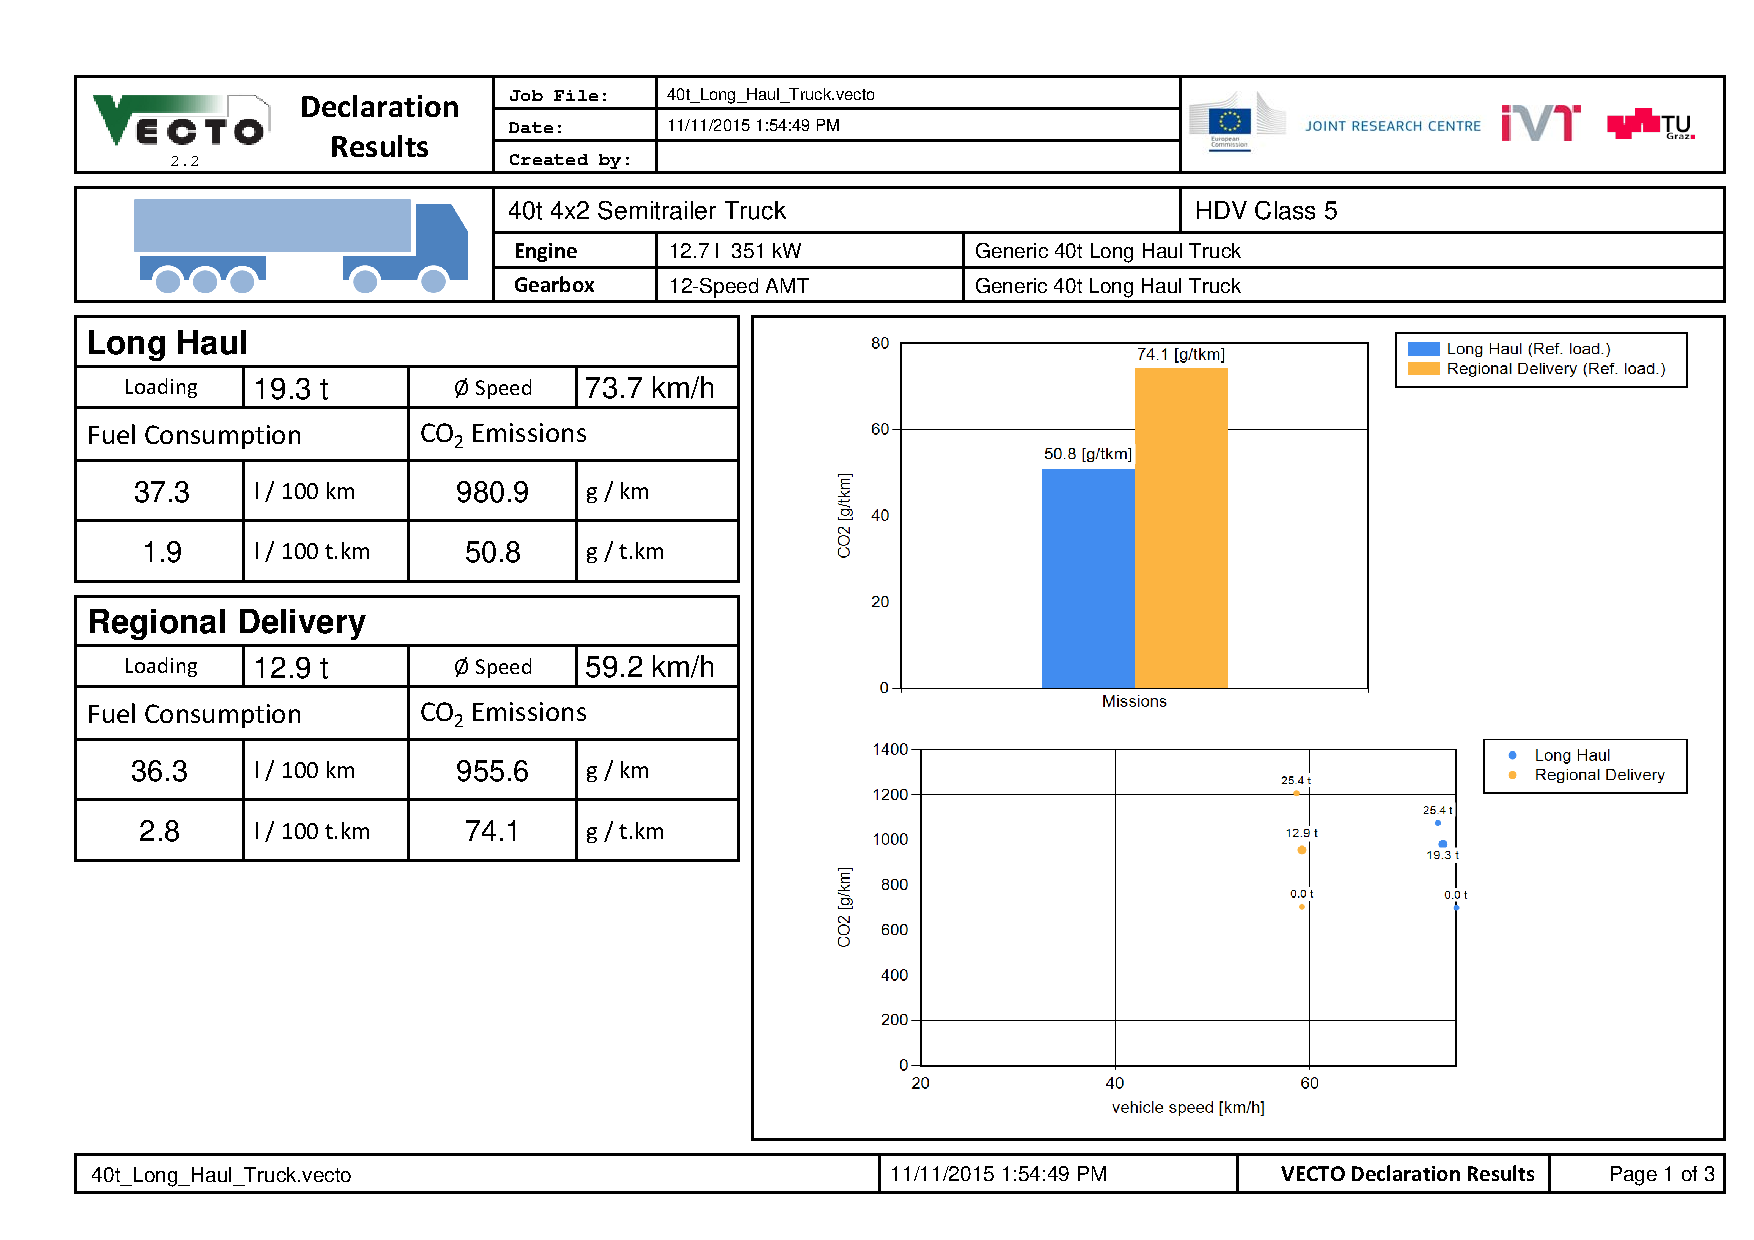
\includepdf[pages=-,scale=0.25,pagecommand=\subsection{Vecto 2.2: 40t Long Haul Truck}\label{sub:vecto_2_2_40t_long_haul_truck}]{img/40t_Long_Haul_Truck_v2}

\fbox{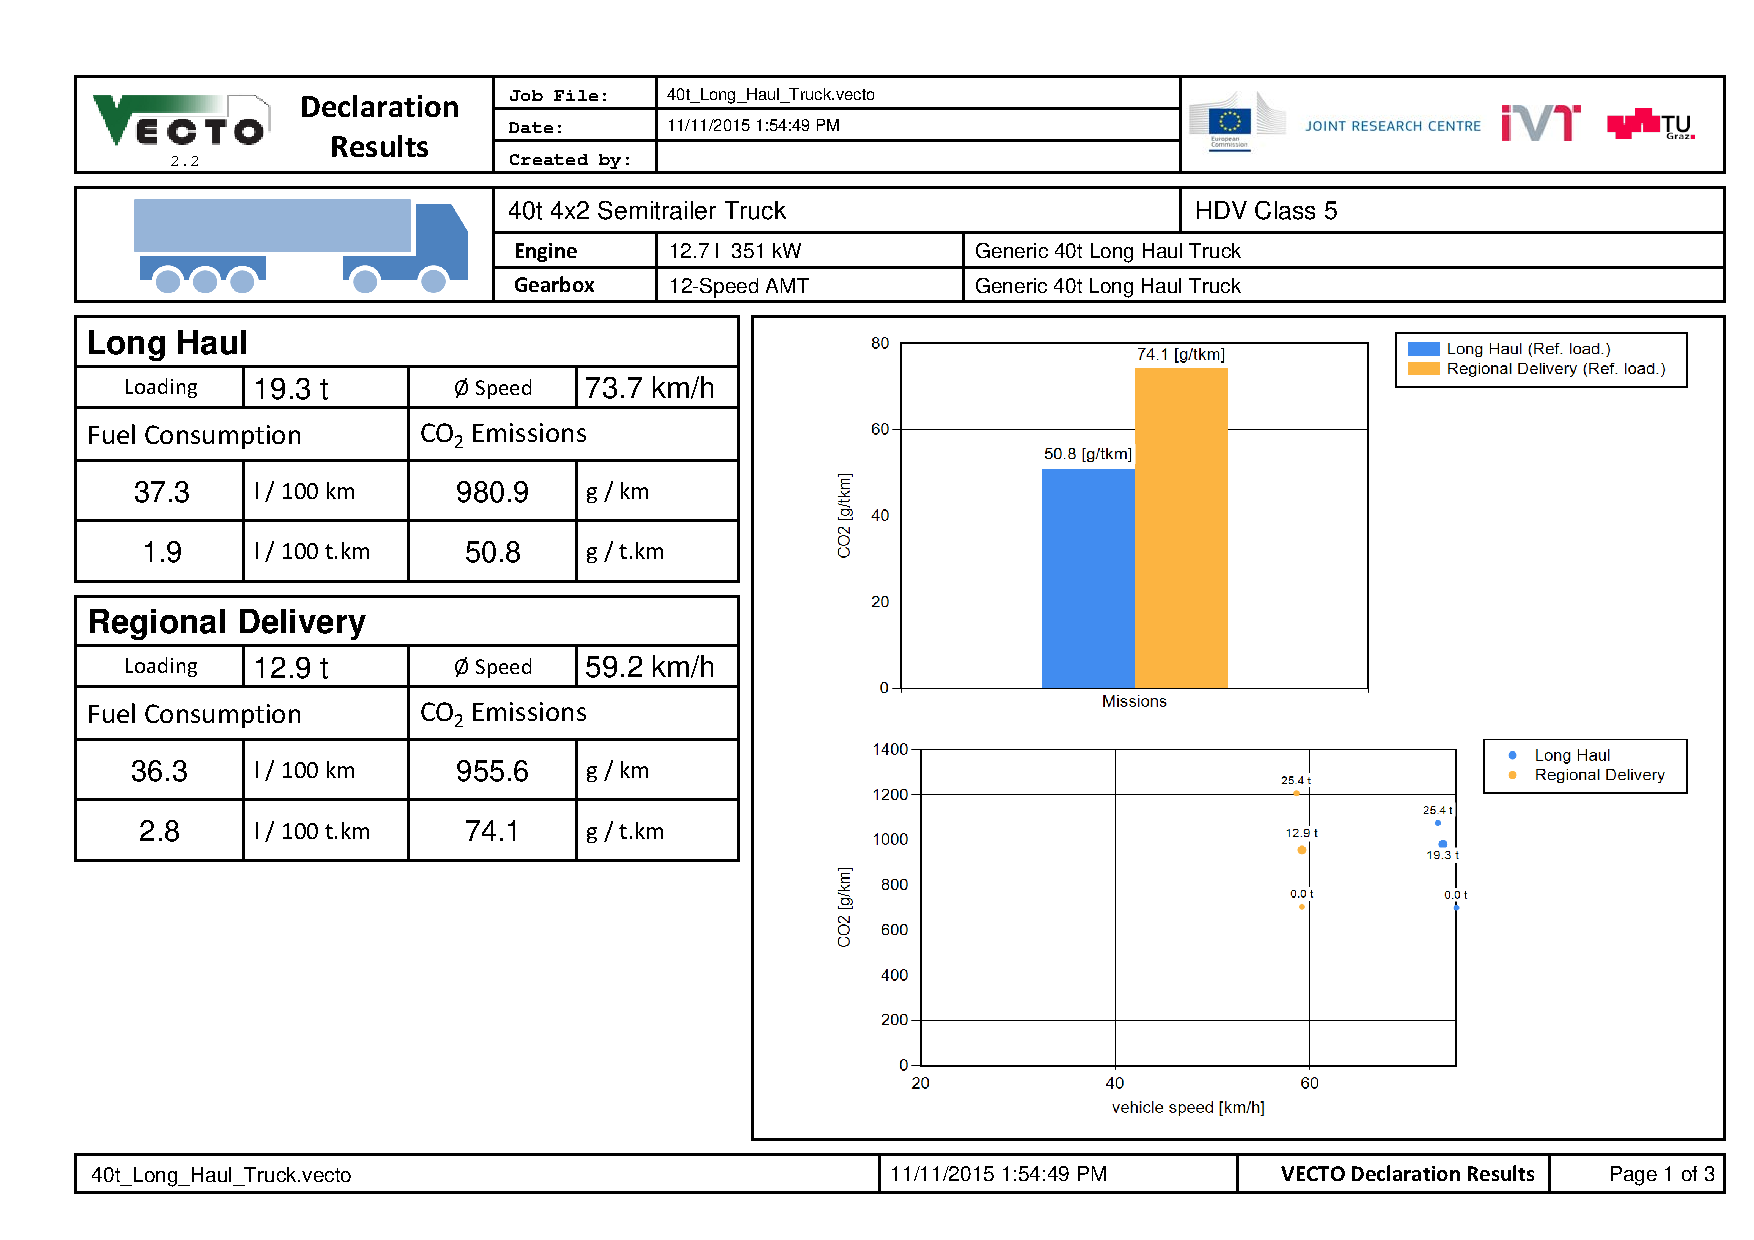
\includegraphics[page=1,scale=0.5]{img/40t_Long_Haul_Truck_v2}}\\[1cm]
\fbox{\includegraphics[page=2,scale=0.5]{img/40t_Long_Haul_Truck_v2}}\\[1cm]
\fbox{\includegraphics[page=3,scale=0.5]{img/40t_Long_Haul_Truck_v2}}

% subsection vecto_2_2_40t_long_haul_truck (end)

%=========================================================================
\subsection{Vecto 3.0.1: 40t Long Haul Truck} % (fold)
\label{sub:vecto_3_0_1_40t_long_haul_truck}
%=========================================================================

\fbox{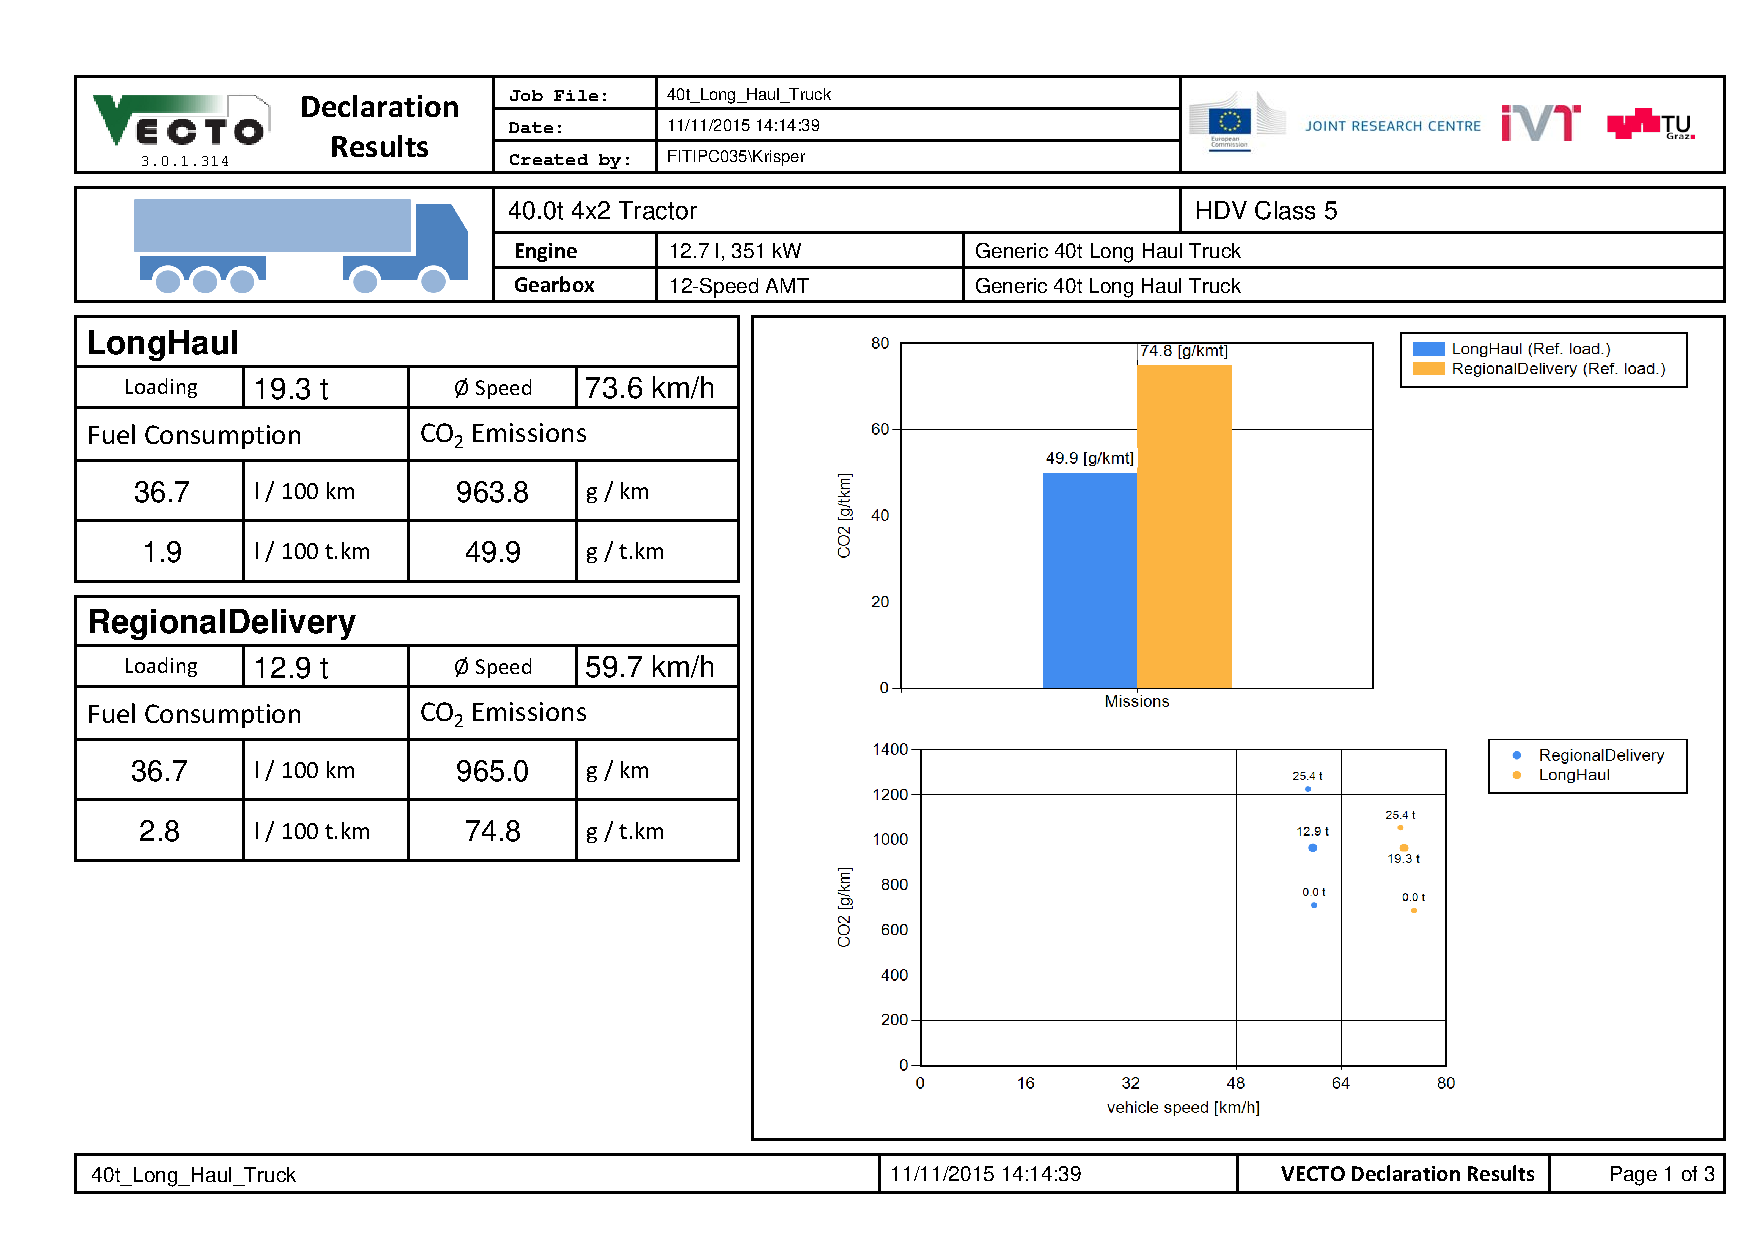
\includegraphics[page=1,scale=0.5]{img/40t_Long_Haul_Truck_v3}}\\[1cm]
\fbox{\includegraphics[page=2,scale=0.5]{img/40t_Long_Haul_Truck_v3}}\\[1cm]
\fbox{\includegraphics[page=3,scale=0.5]{img/40t_Long_Haul_Truck_v3}}

% subsection vecto_3_0_1_40t_long_haul_truck (end)

%=========================================================================
\subsection{Vecto 2.2: 12t Delivery Truck} % (fold)
\label{sub:vecto_2_2_12t_delivery_truck}
%=========================================================================

\fbox{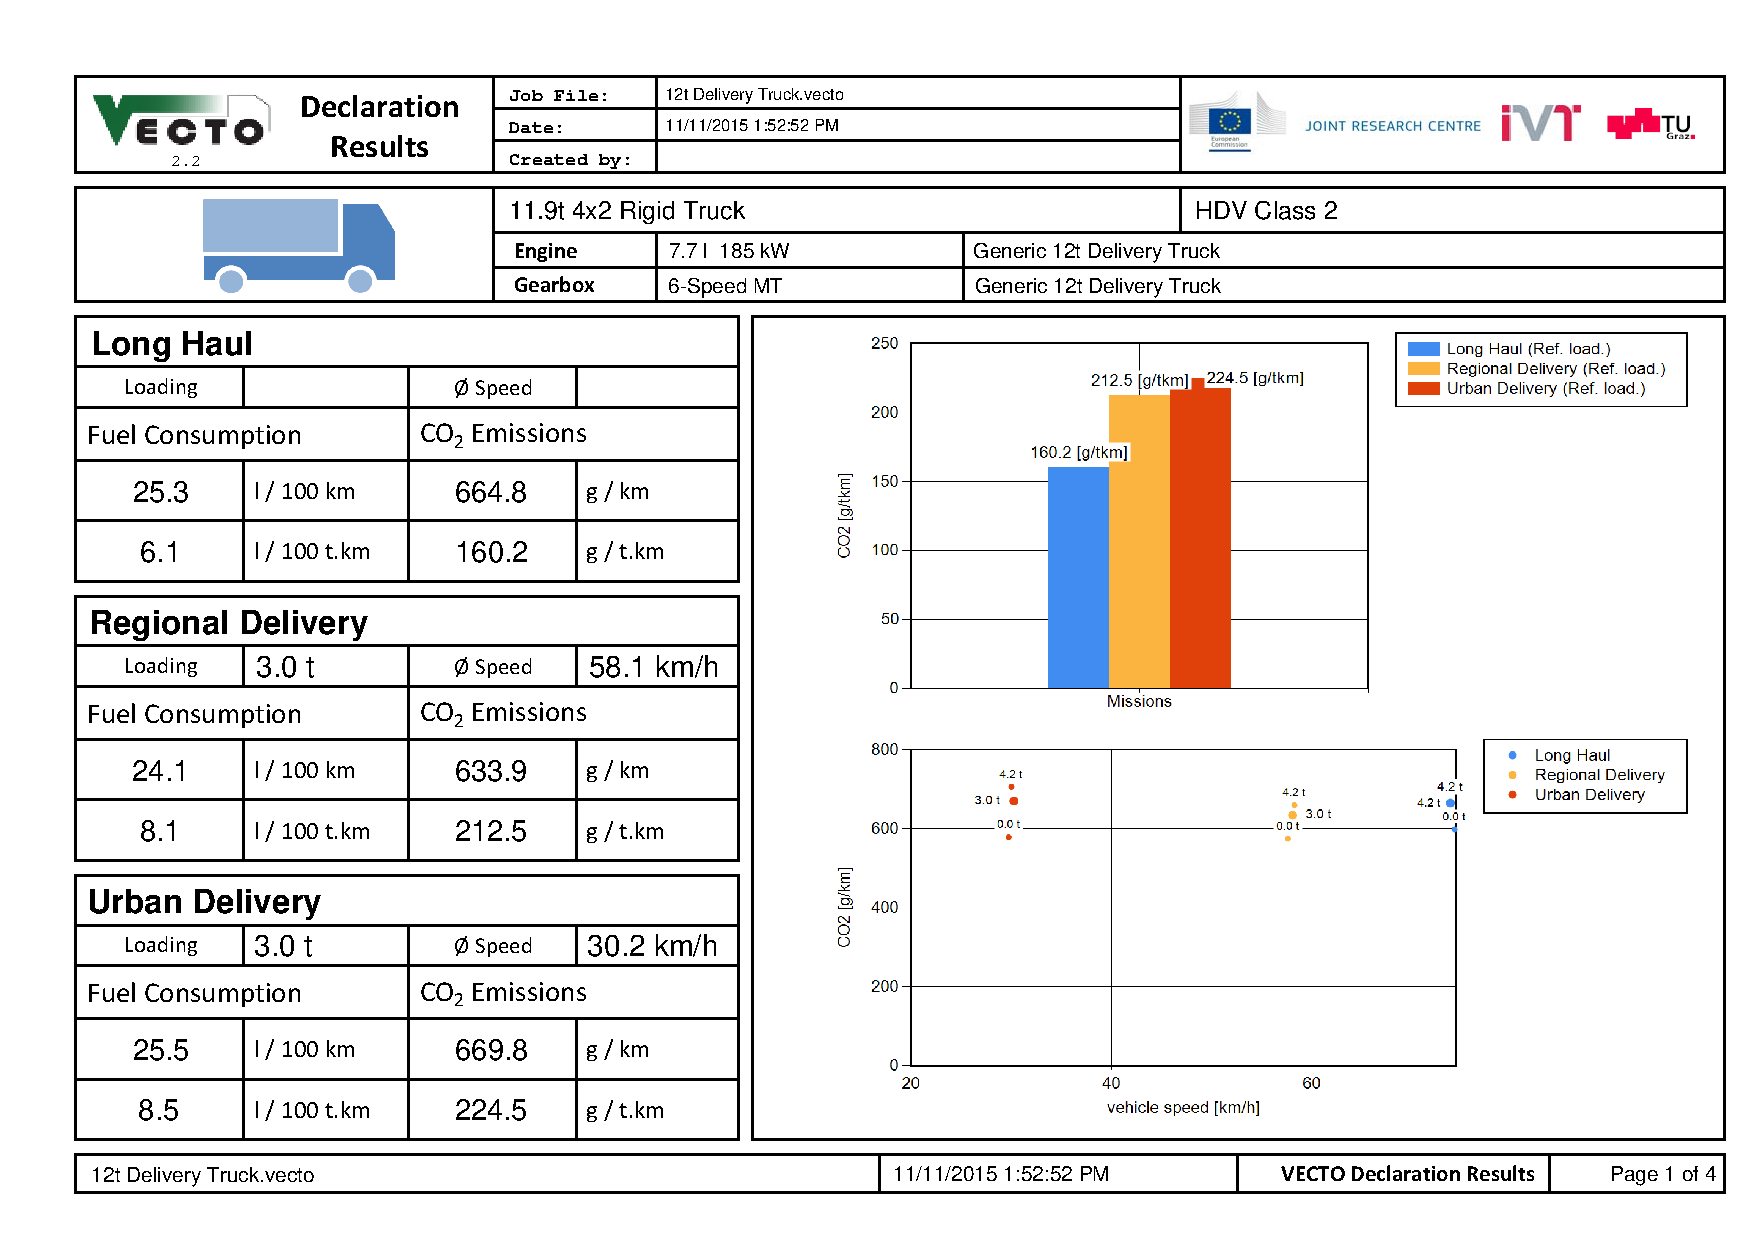
\includegraphics[page=1,scale=0.5]{img/12t_Delivery_Truck_v2}}\\[1cm]
\fbox{\includegraphics[page=2,scale=0.5]{img/12t_Delivery_Truck_v2}}\\[1cm]
\fbox{\includegraphics[page=3,scale=0.5]{img/12t_Delivery_Truck_v2}}

% subsection vecto_2_2_12t_delivery_truck (end)

%=========================================================================
\subsection{Vecto 3.0.1: 12t Delivery Truck} % (fold)
\label{sub:vecto_2_2_12t_delivery_truck}
%=========================================================================

\fbox{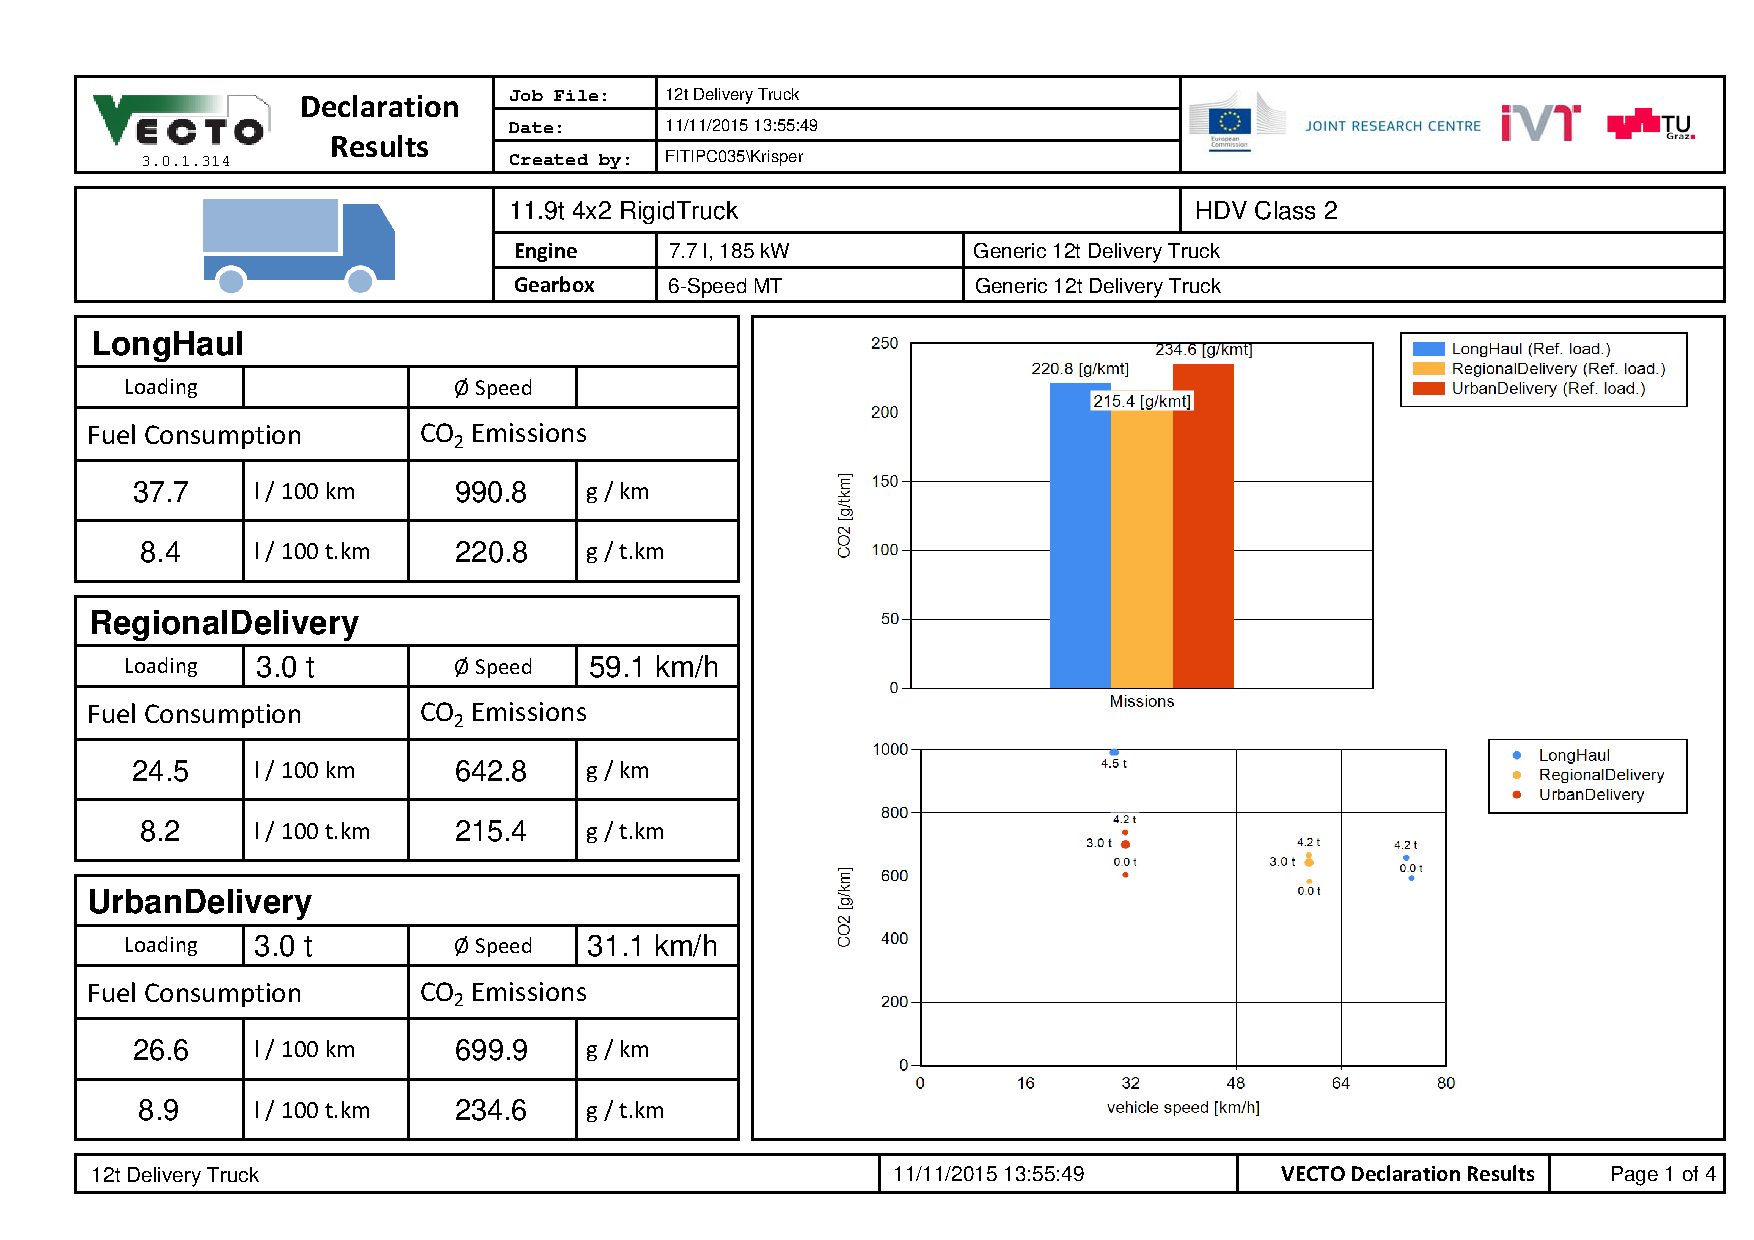
\includegraphics[page=1,scale=0.5]{img/12t_Delivery_Truck_v3}}\\[1cm]
\fbox{\includegraphics[page=2,scale=0.5]{img/12t_Delivery_Truck_v3}}\\[1cm]
\fbox{\includegraphics[page=3,scale=0.5]{img/12t_Delivery_Truck_v3}}

% subsection vecto_2_2_12t_delivery_truck (end)


% section declaration_results_report_for_vecto_2_2_and_vecto_3_0_1 (end)


%----------------------------

% \begin{frame}[t,allowframebreaks]\frametitle{Known Issues}
%     \begin{itemize}
%     	\item 
%     \end{itemize}

% \end{frame}